% !TeX encoding=utf8
% !TeX spellcheck = de-DE

\chapter{Projekt}


\section{Fokus/Ausrichtung}

Das Programm Antz legt einen Schwerpunkt auf die visuelle Veranschaulichung des Ameisenkoloniealgorithmus und das Spiel mit dem Einfluss verschiedener Parameter auf die Lösungsfindung. Funktionell geht es primär um die Lösung des Problems des kürzesten Weges. Allerdings wird mit diesem Programm kein spezifisches Problem wie beispielsweise das TSP effizient gelöst, sondern unterschiedliche Probleme sollen sich rasch lösen können. Die zugrunde liegende Berechnung erfolgt nicht besonders effizient, da dieser Aspekt nicht im Fokus der Entwicklung stand.


% (Animation, Multi-Purpose [kein spezifisches Problem effizient gelöst, sondern mehrere Probleme rasch lösen können]; nicht effiziente Berechnung)

\vspace*{1cm}



\section{Methodisches}


\subsection*{Planung:}

\begin{itemize}[noitemsep]
\item Drei Meilensteine geplant (erster à vier Wochen, zweite à je fünf Wochen)
\item Reserve von zwei Wochen am Ende eingeplant (insgesamt stehen 16 KW zur Verfügung)
\item Abgabe: 30.05.2014
\end{itemize}

\vspace*{1cm}

Vgl. unser Projektplanungstool \\

NB: Eventuell die Besprechungen mit Syrus integrieren (Feedback, Tipps, Stand, etc.) \\


\vspace*{1cm}


\subsection{Hilfsmittel/Planung}

Zur Projektverwaltung und Publikation wurde ein Repository auf GitHub\footnote{\url{https://github.com/jajadinimueter/antz}} verwendet. Dort legten wir auch die wesentlichen Dateien der Dokumentation ab (Ordner «docs»). Für die Planung der Meilensteine und Iterationen wurde das Tool TargetProcess\footnote{\url{http://jajadinimueter.tpondemand.com}} verwendet.


\vspace*{1cm}

Zunächst eröffneten wir einen Account auf sharelatex.com, um gemeinsam an der Projektdokumentation mit LaTeX arbeiten zu können. Später entdeckten wir ein praktisches LaTeX-Template von Matthias Pospiech\footnote{\url{http://www.matthiaspospiech.de/latex/vorlagen/allgemein}}, mit dem die Dokumenation geschrieben werden sollte. Da dafür die Möglichkeiten von sharelatex.com zu wenig ausgeprägt und zu langsam waren, wurde entschieden, die LaTeX-Dokumentation auch mit Git zu pflegen. \\


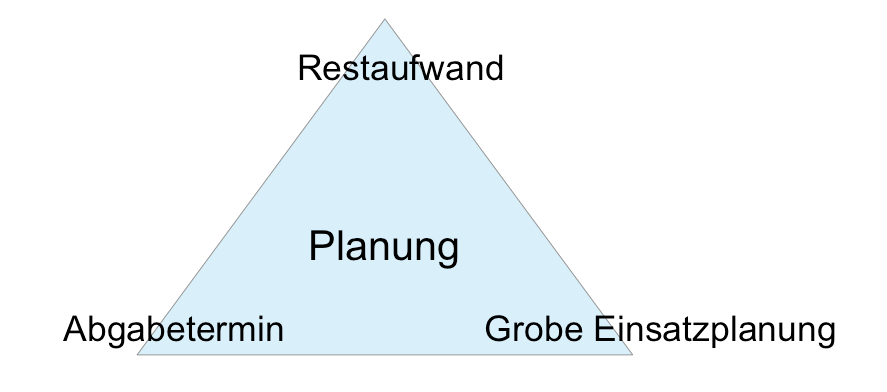
\includegraphics [width=14cm]{images/Planungsdreieck_Quelle.png} 


E-Mail-Kommunikation; regelmässige Treffen \\

TargetProcess, Reporte: Tabellen mit allen Tasks und geplanter/real benötigter Zeit \\

Vgl. Screenshot aus der ersten Folienserie zum Planungsdreieck \\






\section*{Projektplanung}

Evtl. auch offiziellen Zeitplan einbinden \\

Vgl. die Zwischenabgaben (Tabelle ausbauen); Priorisierung; drei Meilensteine \\


\vspace*{1cm}


\section{Technologien}

Gut überlegt \\

Programmiersprache Python, mit Framework pygame (weiter???)

